\begin{figure}[t!]
\centering
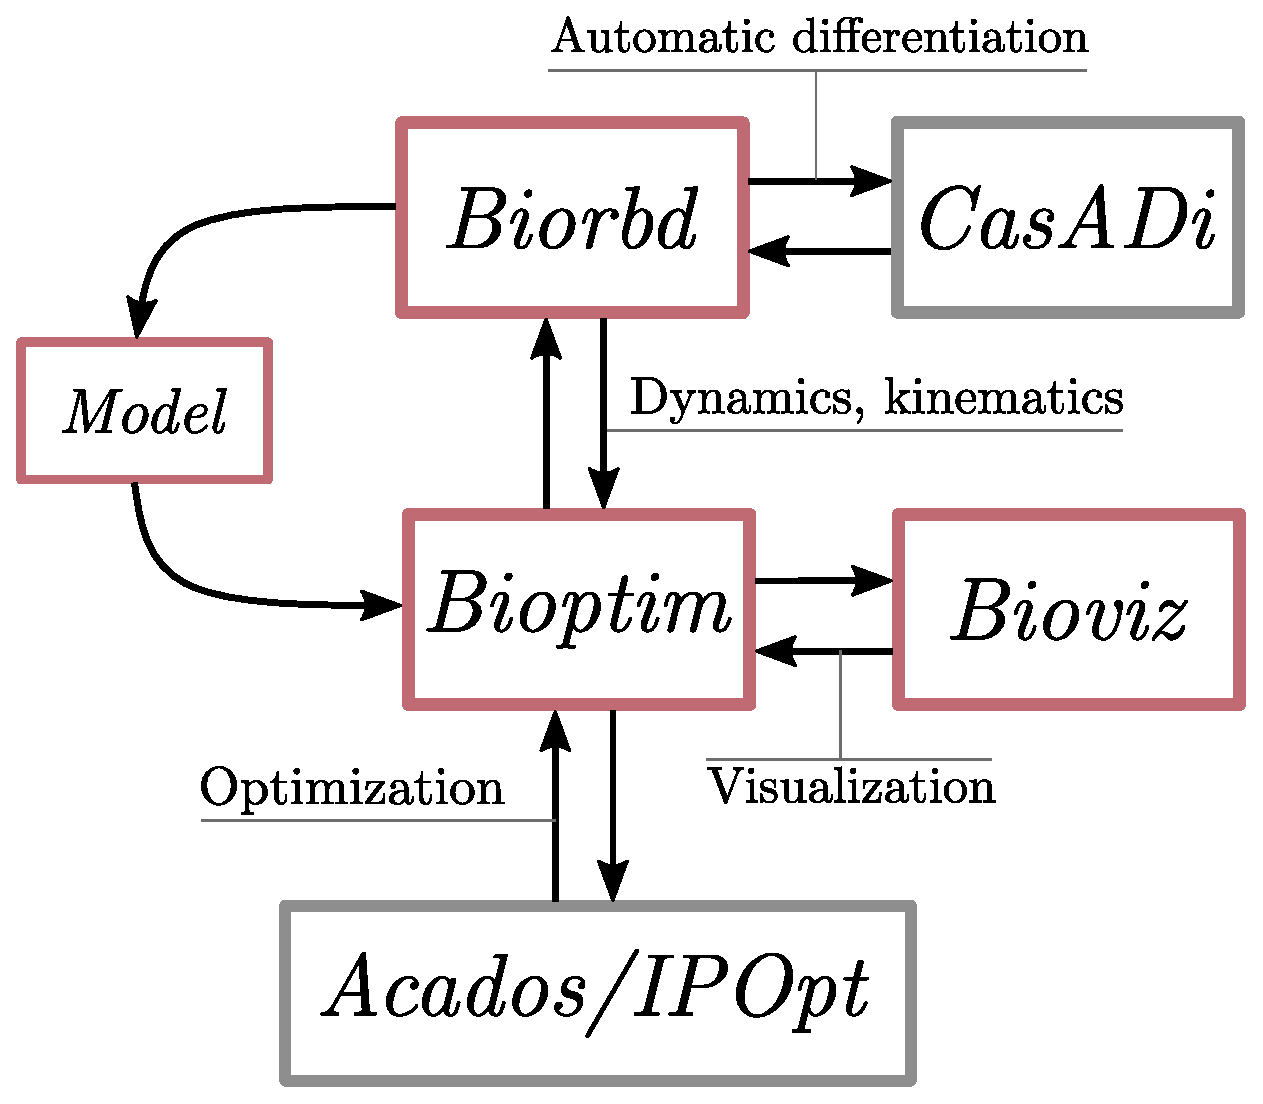
\includegraphics[width=0.9\columnwidth]{figures/dependencies.eps}
\caption{\textit{Bioptim} dependencies flowchart. The red-boxed software are developed by the S2M team.}
\label{fig:dependencies}
\vspace*{-0.5cm}
\end{figure}


\subsection{Implementation and dependencies}

\textit{Bioptim} is the top layer of a succession of software on which it depends to perform various calculations (\textit{Biorbd}: dynamics; \textit{CasADi}: automatic differentiation; \textit{IPOpt, Acados}: optimization; \textit{Bioviz}: visualization).
Within this software bundle, Bioptim's main role is to shape the problem in order to allow its dependencies to communicate efficiently, while providing an intuitive and flexible interface to the user (Fig.~\ref{fig:dependencies}).
Therefore, it was chosen to be written in Python for its flexibility and its widespread use among researchers.
However, all intensive calculations behind the interface are performed in C or C++, keeping it both fast and easy to customize.

\subsection{Design}

Bioptim shapes and solves optimal control problems whose two required entries are a model (.bioMod file) and an OCP. 
The model file contains the geometrical characteristics, the mass and inertia parameters, the geometrical markers and possibly the muscular information of the model. 
It also allows the user to design or import meshes for visualization purposes.
The OCP is implemented as a class whose main attributes are a dynamics type, an objective function, constraints, initial guesses, a number of shooting points and the duration of the problem.
Based on these inputs, \textit{Bioptim} properly sets up the multiple shooting transcription of the OCP and shapes it up to feed the non-linear solver (Ipopt or Acados). 